Luci visitou recentemente o Museu da História da Computação, onde teve a oportunidade de apreciar várias exposições.
Em uma delas, conheceu várias calculadoras antigas como a \emph{Step Reckoner}, criada por volta de 1672.
 Em outra, viu supercomputadores do passado, como os famosos Cray.
 Também conheceu várias maneiras de programar computadores antigos, como cartões perfurados e painéis de tomadas.



Um painel de tomadas em particular chamou a atenção de Luci.
 Nele, há dois blocos com $N$ tomadas cada.
 Em cada bloco, as tomadas são numeradas de $1$ a $N$, da esquerda para a direita.
 Usando uma tecnologia peculiar de cabos, o operador conectava as tomadas de um dos blocos às tomadas do outro bloco.
 Veja o exemplo com $4$ tomadas em cada bloco na figura abaixo.

\begin{figure}[h]
\centering
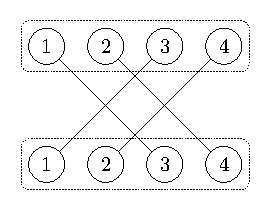
\includegraphics[scale=0.9]{\CWD/images/fig1.pdf}
\end{figure}

Em cada ciclo do computador ao qual esse painel pertence, cada tomada tem  um sinal elétrico que representa um bit.
 O propósito desse painel é trocar a ordem dos bits.
 Por isso, cada tomada de cada bloco deve ser conectada a exatamente uma tomada do outro bloco.
 Cada conexão deve ser feita com um segmento de cabo ligando as duas tomadas em linha reta.
 Por restrições físicas relacionadas à tecnologia peculiar dos cabos, sempre que dois cabos se cruzam o bit transmitido em ambos os cabos muda de valor.
 Ou seja, se o bit 1 estava sendo transmitido por um cabo, este cabo agora passa a transmitir o bit 0.
 No exemplo da figura acima, o cabo conectando a tomada $1$ do bloco superior à tomada $3$ do bloco inferior intercepta dois cabos.
 Dessa forma, o bit transmitido por ele será invertido duas vezes, fazendo com que o bit na tomada $1$ do bloco superior seja o mesmo que o na tomada $3$ do bloco inferior.


Como o objetivo do painel é trocar a ordem dos bits, maneiras de conectar as tomadas que fazem com que o bits em duas tomadas conectadas sejam diferentes não são válidas.
 Ao perceber isso, Luci começou a tentar descobrir de quantas formas era possível conectar as tomadas de maneira válida.
 Ao perceber que o museu tinha vários painéis desses e que, em alguns deles, algumas conexões já haviam sido feitas, ela achou melhor aproveitar o restante da visita ao museu e deixou a pergunta para você: de quantas formas válidas é possível conectar as tomadas, preservando as conexões já existentes?
Lembrando que uma forma é válida se cada tomada estiver conectada a exatamente uma tomada do bloco oposto e se o bit em tomadas conectadas for o mesmo.


\section*{Observações}
\begin{itemize}
\item Se mais de dois cabos se cruzarem em um mesmo ponto, todos os cruzamentos par a par devem ser considerados.

\end{itemize}
\section*{Entrada}

A primeira linha da entrada contém dois inteiros $N$ e $M$, representando o número de tomadas em cada bloco e o número de conexões já existentes respectivamente.

Seguem $M$ linhas, cada uma contendo dois inteiros $a_i$ e $b_i$, indicando que a tomada $a_i$ do bloco superior está conectada à tomada $b_i$ do bloco inferior.


\section*{Saída}

Se $X$ é o número de formas válidas de conectar as tomadas preservando as conexões já existentes, a saída deve conter um único inteiro representado o resto da divisão de $X$ por $1000000007$ ($10^9 + 7$).

 
\section*{Restrições}

\begin{itemize}
\item $1 \leq N \leq 10^6$
\item $0 \leq M \leq 10^6$
\item $1 \leq a_i \leq N$, para todo $i=1,2,\ldots,M$.

\item $1 \leq b_i \leq N$, para todo $i=1,2,\ldots,M$.

\end{itemize}
\section*{Exemplos}
\exemplo
